%
% FROM PROPOSAL:
%

Telehealth (support of health care using electronic information and communication technologies when patient and provider are in a separate location) can play an important role in early detection and treatment of exacerbations. 

In spite of the interest telehealth interventions have gained, studies have produced conflicting results regarding the effectiveness of telehealth interventions \citep{pedone}. One of the factors that may be linked to the cause of telehealth interventions failing to detect exacerbations early, can be addressed to difficulties assessing symptoms through self-report. Previous studies support this finding and further report that binary self-report measures are not always intuitive for patients, who are constantly symptomatic \citep{pedone}. Since physical symptoms are influenced by psychological and individual processes \citep{pennebakker}, self-reported binary measures might be biased and further not capture the relevant features necessary for clinical decision making.  


%
% FROM LONG DRAFT:
%

%
%Chronic Obstructive Pulmonary Disease (COPD) is a progressive lung disease in which the airways are damaged and patients have to cope with various different symptoms, such as shortness of breath (known as dyspnea), phlegm, cough, wheezing and/or chest tightness \cite{Kessler}. Exacerbations  - a worsening in patients’ lung function or symptoms - are a major problem with COPD. Delayed treatment following their onset increased use of healthcare services, readmission to the hospital and a decline in health-related quality of life \cite{Wilkinson}. Early detection and treatment of exacerbations are therefore an important step towards preventing decline in patients’ quality of life and healthcare utilisation.
%
%Telehealth systems that allows for remote monitoring of patients using information and communication technologies are widely used today for the purpose of early detection and treatment of exacerbations in COPD. In telehealth, patients collect both objective (e.g. oxygen saturation) and subjective data (e.g. binary answers to whether there is an increase in dyspnea more than usual). The collected data is transmitted to healthcare providers (usually trained nurses) who review it. Based on an individual “normal range” defined by a healthcare provider, the system flags data for follow-ups in which healthcare providers contact the patient, if needed to advise on potential initiation of treatment. Despite the gained interest in telehealth interventions, studies have produced conflicting results regarding their effectiveness \cite{Pedone}. 


%In the context of chronically ill healthcare providers implement telehealth systems to communicate remotely with patients, when they are out of clinic. Telehealth systems require active participation of patients to collect objective and subjectively assessed data that are directly related to a health condition. While the health domain literature typically focuses only on the comparison of effectiveness of telehealth systems with standard care approaches, literature shows several user needs and concerns that needs to be addressed, when developing self-tracking tools. These user needs have not been investigated in the telehealth domain. We conducted a study on COPD patients who used a state of the art telehealth solution to addresses this gap. 

%While telehealth can be categorized as a form of prescribed self-tracking, it is a special case, given that patients are monitored by a healthcare provider and mandated to self-track. 

\begin{figure}[!h] \centering
			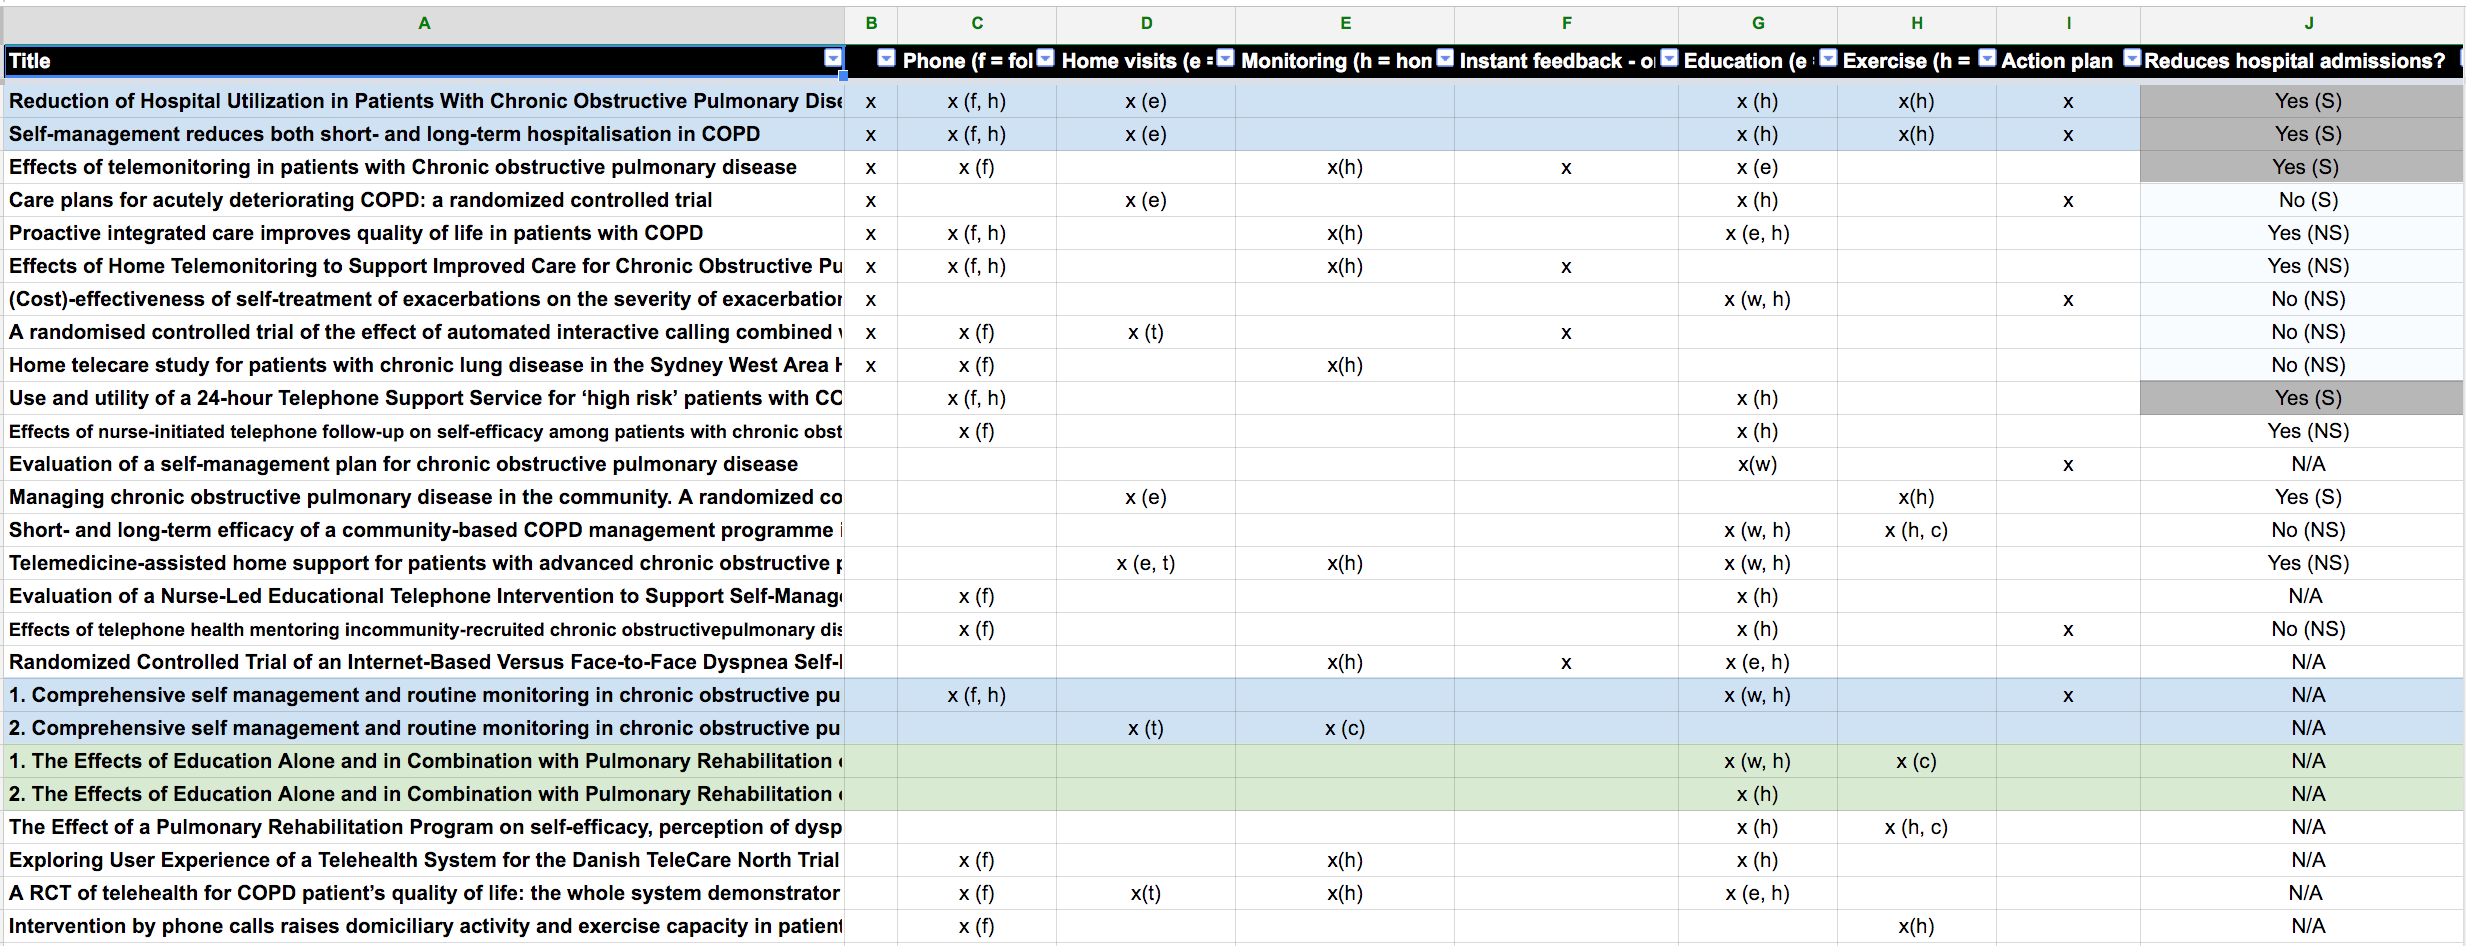
\includegraphics[width=1\textwidth]{Images/telehealth/thInitial.png}
		\caption{Research table with health-related outcomes of telehealth interventions} \label{fig:thInitial}
\end{figure}

\section{Current Literature}
We made an extensive review on telehealth literature and found little on how telehealth systems have been designed to patients needs (See research tables on CD). Current literature primarily shows health-related outcomes of telehealth interventions in comparison with standard care. We compared outcomes from different studies on telehealth studies (See Figure \ref{fig:thInitial}) and found conflicting results due to a wide range of different interventions used. From this it is difficult to assess what has an effect.
